\documentclass[a4paper,12pt]{article}
\usepackage[indonesian]{babel}
\usepackage{graphicx}
\usepackage{multirow}
\usepackage{enumitem}
\usepackage{listings}
\usepackage{wrapfig}
\usepackage[T1]{fontenc}
\usepackage{inconsolata}
\usepackage{lipsum}
\usepackage{adjustbox}
\usepackage{upquote}


\usepackage{color}
\usepackage[table]{xcolor}
\definecolor{lightgray}{rgb}{0.95, 0.95, 0.95}
\definecolor{darkgray}{rgb}{0.4, 0.4, 0.4}
%\definecolor{purple}{rgb}{0.65, 0.12, 0.82}
\definecolor{editorGray}{rgb}{0.95, 0.95, 0.95}
\definecolor{editorOcher}{rgb}{1, 0.5, 0} % #FF7F00 -> rgb(239, 169, 0)
\definecolor{editorGreen}{rgb}{0, 0.5, 0} % #007C00 -> rgb(0, 124, 0)
\definecolor{orange}{rgb}{1,0.45,0.13}		
\definecolor{olive}{rgb}{0.17,0.59,0.20}
\definecolor{brown}{rgb}{0.69,0.31,0.31}
\definecolor{purple}{rgb}{0.38,0.18,0.81}
\definecolor{lightblue}{rgb}{0.1,0.57,0.7}
\definecolor{lightred}{rgb}{1,0.4,0.5}
% CSS
\lstdefinelanguage{CSS}{
  keywords={color,background-image:,margin,padding,font,weight,display,position,top,left,right,bottom,list,style,border,size,white,space,min,width, transition:, transform:, transition-property, transition-duration, transition-timing-function},	
  sensitive=true,
  morecomment=[l]{//},
  morecomment=[s]{/*}{*/},
  morestring=[b]',
  morestring=[b]",
  alsoletter={:},
  alsodigit={-}
}

% JavaScript
\lstdefinelanguage{JavaScript}{
  morekeywords={typeof, new, true, false, catch, function, return, null, catch, switch, var, if, in, while, do, else, case, break},
  morecomment=[s]{/*}{*/},
  morecomment=[l]//,
  morestring=[b]",
  morestring=[b]'
}

\lstdefinelanguage{HTML5}{
  language=html,
  sensitive=true,	
  alsoletter={<>=-},	
  morecomment=[s]{<!-}{-->},
  tag=[s],
  otherkeywords={
  % General
  >,
  % Standard tags
	<!DOCTYPE,
  </html, <html, <head, <title, </title, <style, </style, <link, </head, <meta, />,
	% body
	</body, <body,
	% Divs
	</div, <div, </div>, 
	% Paragraphs
	</p, <p, </p>,
	% scripts
	</script, <script,
  % More tags...
  <canvas, /canvas>, <svg, <rect, <animateTransform, </rect>, </svg>, <video, <source, <iframe, </iframe>, </video>, <image, </image>, <header, </header, <article, </article
  },
  ndkeywords={
  % General
  =,
  % HTML attributes
  charset=, src=, id=, width=, height=, style=, type=, rel=, href=,
  % SVG attributes
  fill=, attributeName=, begin=, dur=, from=, to=, poster=, controls=, x=, y=, repeatCount=, xlink:href=,
  % properties
  margin:, padding:, background-image:, border:, top:, left:, position:, width:, height:, margin-top:, margin-bottom:, font-size:, line-height:,
	% CSS3 properties
  transform:, -moz-transform:, -webkit-transform:,
  animation:, -webkit-animation:,
  transition:,  transition-duration:, transition-property:, transition-timing-function:,
  }
}

\lstdefinestyle{htmlcssjs} {%
  % General design
%  backgroundcolor=\color{editorGray},
  basicstyle={\footnotesize\ttfamily},   
  frame=single,
  % line-numbers
  % Code design
  identifierstyle=\color{black},
  keywordstyle=\color{blue}\bfseries,
  ndkeywordstyle=\color{editorGreen}\bfseries,
  stringstyle=\color{editorOcher}\ttfamily,
  commentstyle=\color{brown}\ttfamily,
  % Code
  language=HTML5,
  alsolanguage=JavaScript,
  alsodigit={.:;},	
  tabsize=2,
  showtabs=false,
  showspaces=false,
  showstringspaces=false,
  extendedchars=true,
  breaklines=true,
  % German umlauts
  literate=%
  {Ö}{{\"O}}1
  {Ä}{{\"A}}1
  {Ü}{{\"U}}1
  {ß}{{\ss}}1
  {ü}{{\"u}}1
  {ä}{{\"a}}1
  {ö}{{\"o}}1
}
%
\lstdefinestyle{py} {%
language=python,
literate=%
*{0}{{{\color{lightred}0}}}1
{1}{{{\color{lightred}1}}}1
{2}{{{\color{lightred}2}}}1
{3}{{{\color{lightred}3}}}1
{4}{{{\color{lightred}4}}}1
{5}{{{\color{lightred}5}}}1
{6}{{{\color{lightred}6}}}1
{7}{{{\color{lightred}7}}}1
{8}{{{\color{lightred}8}}}1
{9}{{{\color{lightred}9}}}1,
basicstyle=\footnotesize\ttfamily, % Standardschrift
numbers=left,               % Ort der Zeilennummern
%numberstyle=\tiny,          % Stil der Zeilennummern
%stepnumber=2,               % Abstand zwischen den Zeilennummern
numbersep=5pt,              % Abstand der Nummern zum Text
tabsize=4,                  % Groesse von Tabs
extendedchars=true,         %
breaklines=true,            % Zeilen werden Umgebrochen
keywordstyle=\color{blue}\bfseries,
frame=b,
commentstyle=\color{brown}\itshape,
stringstyle=\color{editorOcher}\ttfamily, % Farbe der String
showspaces=false,           % Leerzeichen anzeigen ?
showtabs=false,             % Tabs anzeigen ?
xleftmargin=17pt,
framexleftmargin=17pt,
framexrightmargin=5pt,
framexbottommargin=4pt,
%backgroundcolor=\color{lightgray},
showstringspaces=false,      % Leerzeichen in Strings anzeigen ?
}%
%
\definecolor{dkgreen}{rgb}{0,.6,0}
\definecolor{dkblue}{rgb}{0,0,.6}
\definecolor{dkyellow}{cmyk}{0,0,.8,.3}

\lstdefinestyle{PHP}{
  language        = php,
  basicstyle      = \small\ttfamily,
  keywordstyle    = \color{dkblue},
  stringstyle     = \color{red},
  identifierstyle = \color{dkgreen},
  commentstyle    = \color{gray},
  emph            =[1]{php},
  emphstyle       =[1]\color{black},
  emph            =[2]{if,and,or,else},
  emphstyle       =[2]\color{dkyellow}}
\lstset{
    showstringspaces=false,
    frame=single,
    breaklines=true,
    rulecolor=\color{black},
    style=htmlcssjs
}
%

\graphicspath{ {./img/} }
\begin{document}
\title{ {\Large Laporan Praktikum}\\ Pemrograman Web Client\\{\Large Pertemuan 10}}

\author{Aldzikri Dwijayanto Prathama 
	\\195410189
	\\Informatika}
\makeatletter
\begin{titlepage}
	\begin{center}
		{\huge \bfseries \@title }\\[14ex]
		
\includegraphics[scale=.8]{logo}\\[4ex]
		{\large \@author}\\[12ex]
		{\large \bfseries {SEKOLAH TINGGI MANAJEMEN INFORMATIKA DAN KOMPUTER
				AKAKOM YOGYAKARTA}}
	\end{center}


%{\large \@date} 
\end{titlepage}
\makeatother
%\maketitle
\renewcommand{\figurename}{Gambar}
\newpage
\tableofcontents
\newpage
\section{Tujuan}
Menuliskan script javascript menerapkan array, objek, struktur control(if, while, dll), fungsi.
\section{Dasar Teori}

Array pada umumnya adalah sebuah variable yang dapat menampung banyak
value dalam 1 waktu dan untuk mengakses nilai dari array cukup dengan
menentukan index dari arraynya. Dalam JavaScript array memiliki method, sort
dan iteration.\\

Struktur Kontrol dalam JavaScript meliputi JavaScript Condition, Switch, Loop
For, Loop While, dan break. JavaScript condition adalah untuk menentukan
tindakan pada kondisi tertentu.\\

Fungsi atau function dalam JavaScript adalah suatu blok code yang dirancang
untuk melakukan tugas tertentu. Untuk membuat fungsi menggunakan keyword
function.\\

Objek dalam JavaScript adalah suatu tipe data yang didefinisikan sebagai
mutable properties collection, yang artinya sekumpuluan properti (ciri khas) yang
nilainya dapat berubah. Dengan JavaScript dapat mudah untuk membuat objek
sendiri.\\
\newpage

\section{Pembahasan}
\subsection{Praktik}
\subsubsection{Praktik 1}
\textbf{Membuat Array\\}
\begin{lstlisting}[style=htmlcssjs]
<!DOCTYPE html>
<html>
    <body>
        <h2>Javascript Array</h2>
        <p>STMIK AKAKOM</p>
        <p id="demo"></p>
   <script>
       var jurusan = ["Manajemen Informatika",
           "Komputer Akuntansi",
           "Teknik Komputer",
           "Teknik Informatika",
           "Sistem Informasi"];
       document.getElementById("demo").innerHTML = jurusan;
   </script>
    </body>
</html>
\end{lstlisting}
Dokumen html pada praktik pertama memiliki variabel yang bertipe array, yang dideklarasikan dengan var. Kemudian isi
dari variabel array tersebut dicetak pada element dengan id demo.
\begin{center}
    
\includegraphics[scale=.7]{1.png} 
\end{center}

\subsubsection{Praktik 2}
\textbf{JavaScript If Condition}
\begin{lstlisting}
<!DOCTYPE html>
<html>
    <body>
        <p>Javascript If Condition</p>
        <p id="demo"></p>
   <script>
       var angka = 10;
       if (angka < 15) {
           hasil = "angka lebih kecil dari 15";
       }
       else {
           hasil = "angka lebih besar dari 15";
       }
       document.getElementById("demo").innerHTML=hasil;
   </script>
    </body>
</html>
\end{lstlisting}
Dokumen html tersebut memiliki script javascript dengan if condition. Pernyataan if akan mengecek apakah bilangan yang
berada di dalam variabel angka bernilai lebih kecil atau lebih besar dari 15. Jika nilai pada variabel angka lebih kecil
dari 15, maka variabel hasil akan diisi string "angka lebih kecil dari 15", tetapi jika nilai pada variabel angka lebih
besar maka variabel hasil akan diisi string "angka lebih besar dari 15". Kemudian variabel hasil akan dicetak.

\begin{center}
    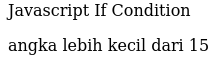
\includegraphics[scale=.7]{2.png} 
\end{center}

\subsubsection{Praktik 3}
\textbf{JavaScript Switch}
\begin{lstlisting}
<!DOCTYPE html>
<html>

<body>
    <p id="demo"></p>
    <script>
        var day = 4;
        switch (day) {
            case 0:
                day = "Sunday";
                break;
            case 1:
                day = "Monday";
                break;
            case 2:
                day = "Tuesday";
                break;
            case 3:
                day = "Wednesday";
                break;
            case 4:
                day = "Thursday";
                break;
            case 5:
                day = "Friday";
                break;
            case 6:
                day = "Saturday";
        }
        document.getElementById("demo").innerHTML = "Today is " + day;
    </script>
</body>

</html>

\end{lstlisting}

Javascript pada html tersebut memiliki seleksi switch case, yang berisi nama-nama hari dalam seminggu. Karena nilai pada
variabel day bernilai 4, berarti akan masuk ke case 4, dan variabel day nilainya berubah menjadi ``Thursday''.
\begin{center}
    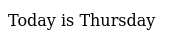
\includegraphics[scale=.7]{3.png} 
\end{center}

\subsubsection{Praktik 4}
\textbf{JavaScript Loop For\\}
\begin{lstlisting}
<!DOCTYPE html>
<html>

<body>
    <h2>Javascript For Loop</h2>
    <p id="demo"></p>
    <script>
        var cars = ["BMW", "Volvo", "Saab", "ford", "Fiat", "Audi"];
        var text = "";
        var i;
        for (i = 0; i < cars.length; i++) {
            text += cars[i] + "<br>";
        }
        document.getElementById("demo").innerHTML = text;
    </script>
</body>

</html>
\end{lstlisting}
Script javascript pada dokumen html tersebut memiliki loop for, yang dimulai dari 0. Didalamnya terdapat pernyataan yang
berguna untuk memindahkan nilai array pada variabel cars ke text secara satu persatu.

\begin{center}
    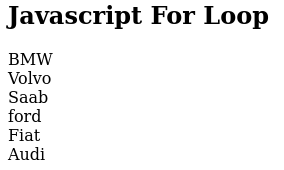
\includegraphics[scale=.7]{4.png} 
\end{center}

\subsubsection{Praktik 5}
\textbf{JavaScript Loop While\\}
\begin{lstlisting}
<!DOCTYPE html>
<html>

<body>
    <h2>Javascript While Loop</h2>
    <p id="demo"></p>
    <script>
        var text = "";
        var i = 0;
        while (i < 10) {
            text += "<br> The number is " + i;
            i++;
        }
        document.getElementById("demo").innerHTML = text;
    </script>
</body>

</html>
\end{lstlisting}

Untuk script javascript selanjutnya memiliki perulangan while yang akan berjalan selama variabel i memiliki nilai kurang
dari 10. Di dalam perulangan while terdapat pernyataan untuk mengisi variabel text dengan array, dan increment terhadap
variabel i.

\begin{center}
    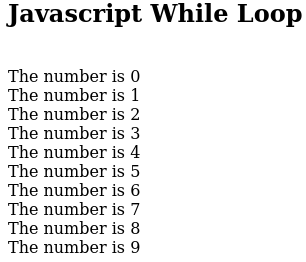
\includegraphics[scale=.7]{5.png} 
\end{center}

\subsubsection{Praktik 6}
\textbf{JavaScript Functions\\}
\begin{lstlisting}
<!DOCTYPE html>
<html>

<body>
    <h2>Javascript Functions</h2>
    <p>Contoh Penggunaan fungsi untuk perkalian</p>
    <p id="demo"></p>

    <script>
        var x = myFunction(4, 3);
        document.getElementById("demo").innerHTML = x;

        function myFunction(a, b) {
            return a * b;
        }
    </script>

</body>

</html>
\end{lstlisting}

Praktik selanjutnya adalah membuat praktik pada javascript, fungsi myFunction memiliki parameter a dan b, dan di
dalamnya terdapat operasi perkalian antara a dengan b. fungsi myFunction dipanggil pada pada deklarasi variabel x,
dengan parameter 4 dan 3, sehingga variabel x berisi hasil dari perkalian antara 4 dengan 3.

\begin{center}
    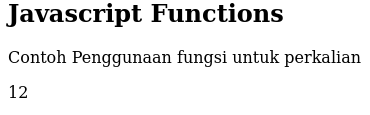
\includegraphics[scale=.7]{6.png} 
\end{center}

\subsubsection{Praktik 7}
\textbf{JavaScript Objects\\}
\begin{lstlisting}
<!DOCTYPE html>
<html>

<body>
    <p>Creating a Javascript Object.</p>
    <p id="demo"></p>
    <script>
        var person = {firstName: "John", lastName: "Doe", age: 50, eyeColor: "blue"};
        document.getElementById("demo").innerHTML =
            person.firstName + " is " + person.age + " years old.";
    </script>
</body>

</html>
\end{lstlisting}

Praktik 7 adalah membuat objek pada javascript, objek tersebut berisi nama awal, nama akhir, umur, dan warna mata.
Kemudian objek tersebut di cetak pada halaman web.

\begin{center}
    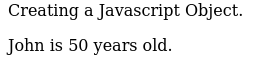
\includegraphics[scale=.7]{7.png} 
\end{center}

\newpage

\subsection{Latihan}
\subsubsection{Latihan 1}
\begin{lstlisting}
<!DOCTYPE html>
<html>
    <body>
        <h2>Javascript Array</h2>
        <p>STMIK AKAKOM</p>
        <p id="demo1"></p>
        <p id="demo2"></p>
   <script>
       var binatang = ["Gajah","Merpati","Anjing","Kucing","Semut"]
       var sayuran = ["Bayam","Tomat","Kacang Panjang","Timun","Kubis"];
       document.getElementById("demo1").innerHTML = binatang;
       document.getElementById("demo2").innerHTML = sayuran;
   </script>
    </body>
</html>
\end{lstlisting}

Pada latihan, mahasiswa membuat variabel array yang berisi nama-nama sayuran dan binatang, yang kemudian di tampilkan
pada halaman web.

\begin{center}
    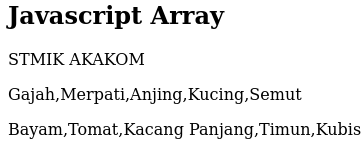
\includegraphics[scale=.7]{8.png} 
\end{center}

\subsubsection{Latihan 2}
\begin{lstlisting}
<!DOCTYPE html>
<html>

<body>
    <p>Creating a Javascript Object.</p>
    <p id="demo"></p>
    <script>
        var person = {firstName:"Aldzikri", lastName:"Prathama", age: 19, eyeColor:"black"};
        document.getElementById("demo").innerHTML =
            person.firstName + " is " + person.age + " years old.";
    </script>
</body>

</html>
\end{lstlisting}

Untuk latihan 2 mahasiswa memodifikasi object pada praktik 7, sehingga menampilkan data diri dari mahasiswa.

\begin{center}
    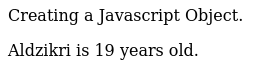
\includegraphics[scale=.7]{9.png} 
\end{center}

\newpage

\section{Kesimpulan}
Setelah praktik, mahasiswa mampu menuliskan script javascript menerapkan array, objek, struktur control (if, while, dll), fungsi.

\end{document}
